% Copyright (c) 2014,2016 Casper Ti. Vector
% Public domain.

\chapter{实验和分析} \label{chap:experiments}
在现有的公开数据集(比如LDBC 、SNAP 、LAW )中,并没有富含重边的场景,这些图也不是属性图。富含重边的属性图普通存在于电信、金融、刑侦等行业中,数据是不公开的。由于实际的数据只能在相关部门内部查询,明略数据根据客户数据中统计出的特征构造测试用图,以支持SCOPA的开发与测试,验证HybriG架构的优秀性能。

本组实验选用的图中有20万个顶点,48197700条边,平均度数为482,每个点平均与3.6个点相邻,两点间同label的重边的平均重数为134。实验对比的是直接将图存储在Titan中的传统方案以及将图存储在HybriG中的方案。

实验环境为5台服务器组成的集群,每台机器安装Ubuntu14.04操作系统,物理配置均为一个Intel Xeon E3-1220 (3.10GHz)处理器、16GB内存、一个1Gbps网卡及一个4TB SATA接口硬盘。HBase部署在这5台机器上,每台机器的RegionServer设置最大堆内存为4GB。其中HBase版本为1.0.1.1,Titan版本为0.5.4。

\section{邻域点集相关查询}
邻域点集查询是指查询给定点的邻接点集。许多图查询基于邻域点集查询实现,如k-hop点集查询、局部聚集系数查询、广度优先搜索等。下面叙述两个基于邻域点集查询的图查询实验。
\subsection{k-hop点集查询}
k-hop点集查询即查询给定点在k跳能到达的点集。实验在测试图中随机抽取100个点作为起点,查询它们的多跳邻域点集,测试它们的平均查询时间。同时又对小邻域(邻域点数小于5)的点集和大邻域(邻域点数大于20)的点集进行了同样的实验。表\ref{khop_random}、表\ref{khop_min}、表\ref{khop_max} 是Titan与HybriG的性能表现。
\begin{table}[!hbp]
\centering
\begin{tabular}{|c|c|c|c|c|}
\hline
\diagbox{架构}{hops} & 1 & 2 & 3 & 4\\
\hline
Titan&13.65&72.97&446.34&2755.86\\
\hline
HybriG&4.25&18.73&34.69&99.78\\
\hline
\end{tabular}
\caption{随机选100个点的k-hop查询平均耗时(毫秒)}
\label{khop_random}
\end{table}

\begin{table}[!hbp]
\centering
\begin{tabular}{|c|c|c|c|c|}
\hline
\diagbox{架构}{hops} & 1 & 2 & 3 & 4\\
\hline
Titan&8.67&31.08&179.47&1140.0\\
\hline
HybriG&2.08&7.79&19.88&52.45\\
\hline
\end{tabular}
\caption{随机选100个小邻域点的k-hop查询平均耗时(毫秒)}
\label{khop_min}
\end{table}

\begin{table}[!hbp]
\centering
\begin{tabular}{|c|c|c|c|c|}
\hline
\diagbox{架构}{hops} & 1 & 2 & 3 & 4\\
\hline
Titan&17.79&110.34&721.25&4781.79\\
\hline
HybriG&3.52&14.49&39.98&163.15\\
\hline
\end{tabular}
\caption{随机选100个大邻域点的k-hop查询平均耗时(毫秒)}
\label{khop_max}
\end{table}
可以看到,随着跳数的增加,两系统的查询时间都呈指数增长。HybriG不管在1跳的初始值还是在增长的倍数上都远优于Titan。正如2.3节分析的,对某个点的邻域点集查询需要遍历该点的邻接表。当图中的重边数目巨大时,Titan受累于其庞大的邻接表,对邻域点集的查询速度大大降低。而HybriG由于极大简化了存储在Titan中的边数目,使得邻接表的数据量大大缩小,从而降低了邻接表的遍历耗时。

\subsection{局部聚集系数计算}
局部聚集系数(Local Cluster Coefficient)是图中每个点的一种度量,用于表示其邻域子图的紧密程度,即邻居节点之间有多大比例有边相连。简要的计算公式如下:
$$LCC(v) = \frac{\left | \left \{(u,w):u,w \in{N_v}, e(u,w)\in{E} \right \} \right |}{\left | \left \{(u,w):u,w\in N_v\right \} \right |}$$
其中$N_v$表示点$v$的邻域点集,$E$表示图中的边集。上式表示邻域的点对集合中,有边相连的点对比例。由于$e(u,w)\in{E}$等价于$w\in{N_u}$,故上式分子部分可转化为
$$\left | \left \{ (u,w):u,w\in{N_v},w\in{N_u} \right \} \right | = \sum_{u\in{N_v}}{\left | N_u \cap N_v  \right |}$$
从上式可知,局部聚集系数的计算需要对邻域点集中的点再做一次邻域点集查询,因此其复杂度相当于2跳邻域点集查询。

\begin{figure}[htbp]
\centering
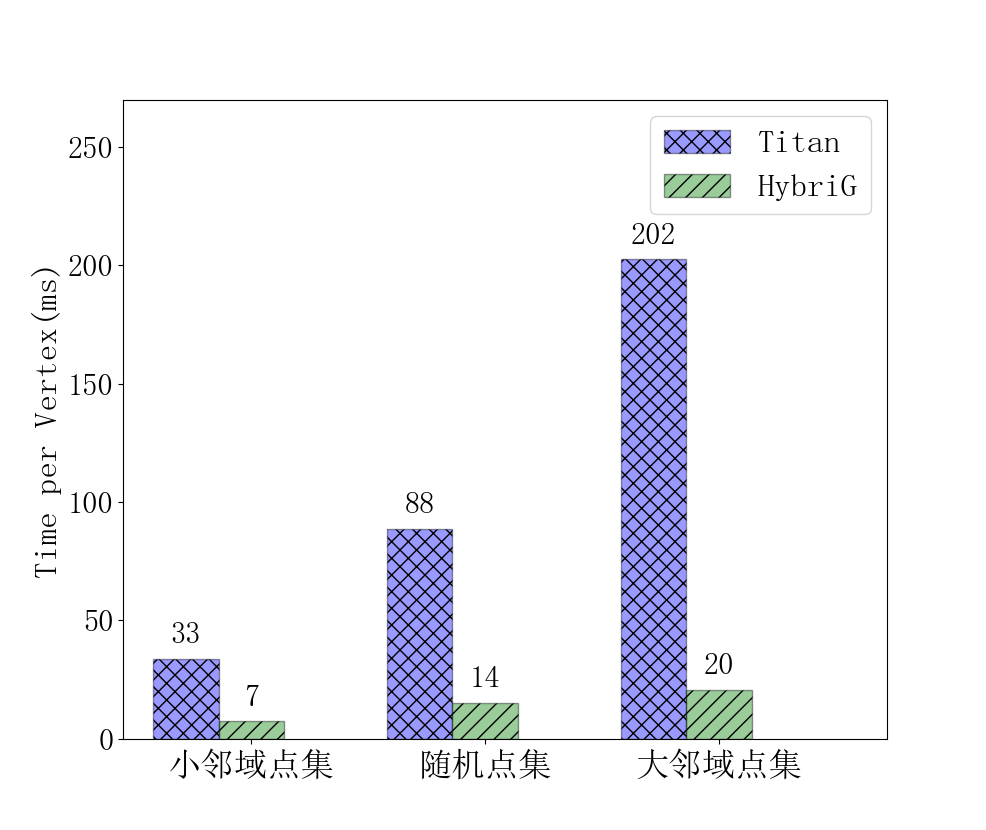
\includegraphics[width=120mm]{fig/local_cc.png}
\caption{计算100个点的局部聚集系数的平均耗时}
\label{fig:local_cc}
\end{figure}

实验对比的是HybriG与直接将图存储在Titan中的传统方案。测试点集的抽取方式同7.1节,即小邻域(邻域点数小于5)的点集、随机采样点集和大邻域(邻域点数大于20)的点集,每个点集拥有100个点。图\ref{fig:local_cc}是实验结果。
与k-hop查询一样,HybriG在局部聚集系数计算的性能上要远优与Titan,而且在大邻域点集上的优势更加明显。

\section{边集相关查询}
下面介绍边集相关查询的两个实验结果。7.2.1节是两点间边集查询,在刑侦场景中,图中的一类顶点代表人,人之间的边代表两人的关系,比如共同出行记录、共同住宿酒店记录、通话记录等。当研判专家锁定两个嫌疑人后,需要查询两人间的关系数据,即为两点间边集查询。7.2.2节是邻接边集查询,在刑侦场景中,锁定嫌疑人后要查看其某种类型的关系数据,即为邻接边集查询。这两种查询的图查询语句是不同的,前者限定了边的两个邻接点,后者只给定了边一个端点,侧重于限定label。使用Blueprints图查询接口,两点间边集查询的示例语句如下:
\begin{center}
  v1.query().adjacent(v2).edges()
\end{center}
邻接边集查询的示例语句如下:
\begin{center}
  v.getEdges(Direction.BOTH, eLabel)
\end{center}
其中v1、v2、v是顶点,eLabel是边的一种label,Direction.BOTH是常量,代表边的方向可以是入边或出边。
\subsection{两点间边集查询}
实验测试的是给定两个点和一个label,查询两点间该label的所有边。在图中随机抽取100个有边相连的点对,实验测试查询这些边的耗时。

\begin{figure}[htbp]
\centering
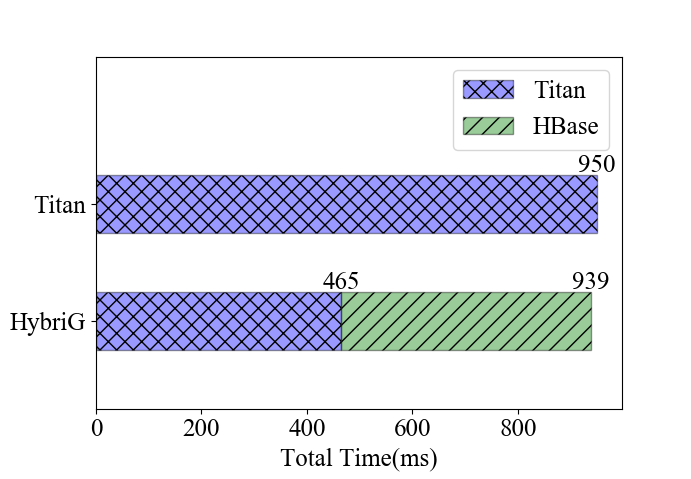
\includegraphics[width=120mm]{fig/edge_query_perf.png}
\caption{查询100个点对间所有边的总耗时}
\label{fig:edge_query_perf}
\end{figure}

图\ref{fig:edge_query_perf}统计了两种系统的时间对比,两种方案的查询耗时非常接近。HybriG的存储层基于Titan和HBase实现,对边集的查询先要在Titan里查询边id,再在HBase的边表中查询具体的边,因此时间开销分两部分(详见5.1节)。图中展示了HybriG查询时间的两部分组成。两种方案的耗时相近主要有两方面的原因。

一方面,HybriG检索边集数据需要在Titan和HBase这两个数据库中进行查询,且这两个查询不能并行。传统方案只需要在Titan中查询,HybriG多加了一轮查询的时间开销。然而,这部分的时间开销并不是很大。Titan的数据表本身也存储在HBase中,HybriG的查询实际上只是HBase中的跨表查询。跨表查询能共用HBase的一些缓存信息,如HMaster、RegionServer的位置信息、HBase中Root表和Meta表的信息等。不过尽管只是跨表查询,在这方面HybriG还是引入了时间开销。
但另一方面,HybriG对边集的查询是转化为HBase边表中的行级别检索(详见5.1节)。而将图存储在Titan中的方案,对边集的查询实际是转化为HBase数据表中选定行后的列级别检索。当图中含有大量重边时,前者是在一张高窄(tall-narrow)表中查找连续的几行,后者是在一张扁宽(flat-wide)表中选定一行后查找连续的几列,前者的性能会略优一些。因此在这方面HybriG略优。


\subsection{邻接边集查询}
实验测试的是给定一个点,查询其某种label的所有边。点集的抽取方式同7.1节,即小邻域(邻域点数小于5)的点集、随机采样点集和大邻域(邻域点数大于20)的点集,每种点集抽取1000个点。

\begin{figure}[htbp]
\centering
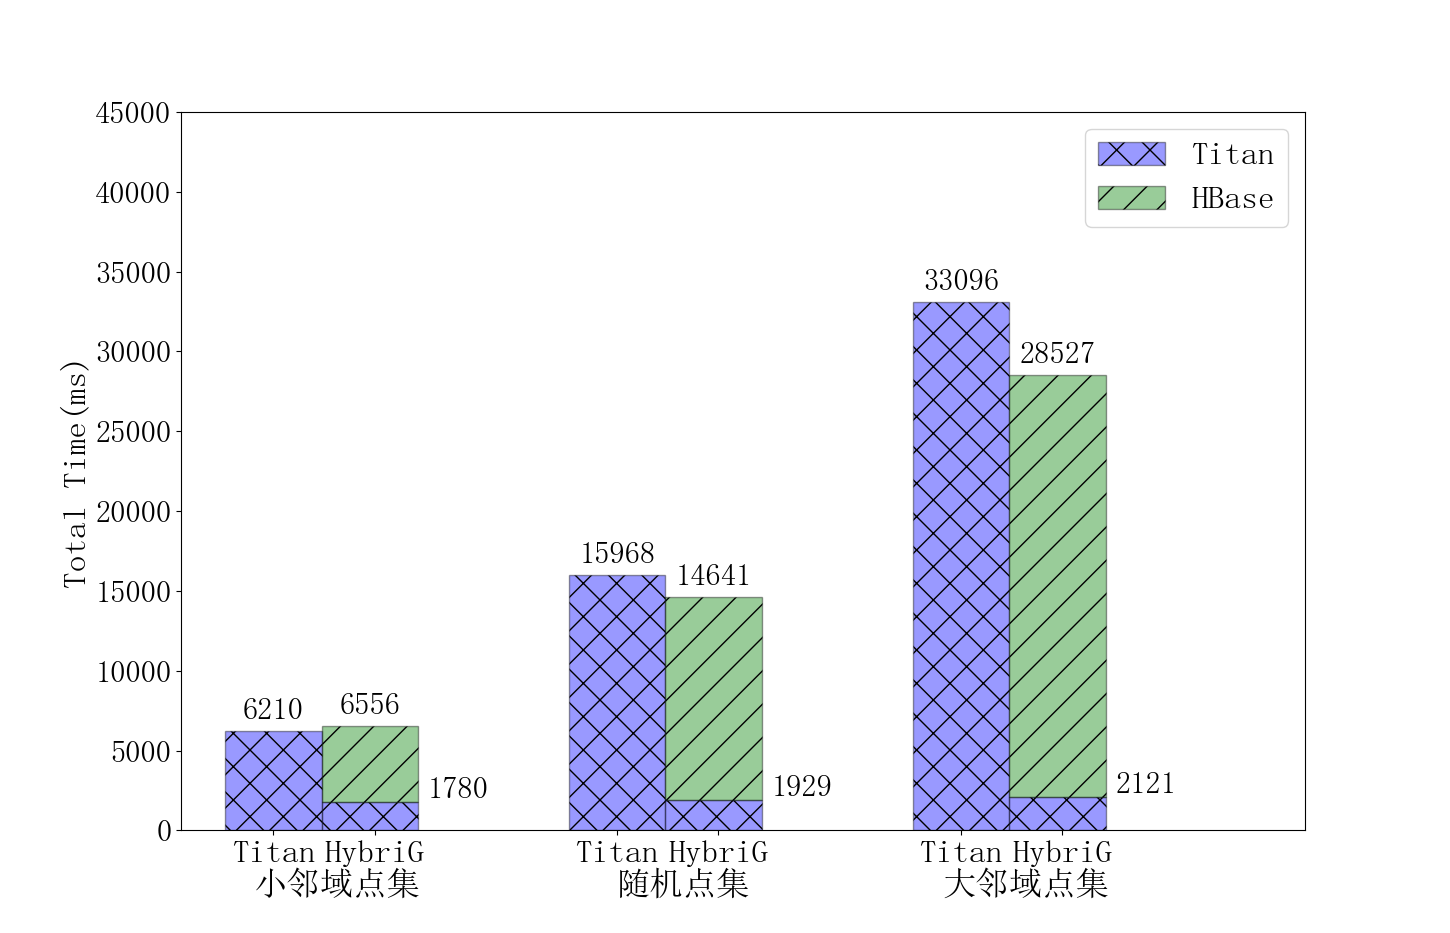
\includegraphics[width=140mm]{fig/get_edges.png}
\caption{查询1000个点给定label的所有边总耗时}
\label{fig:get_edges}
\end{figure}

图\ref{fig:get_edges}展示的是两种系统的查询时间,以及查询耗时中具体的时间组成,其中HybriG的查询时间分为Titan中的查询耗时和HBase中的查询耗时两部分。当边集规模增大时,HybriG在Titan中的查询耗时并没有显著增加,而在HBase边表中的查询耗时增长的幅度也没有传统方案中的Titan大。

\section{边数据的导入速度}
关于边的数据导入速度,我们对不同规模的图进行了测试。对比直接将图存储在Titan以及将图存储在HybriG的两种方案。我们基于MapReduce\supercite{mapreduce}开发了分布式的导入程序。表\ref{edge_load_perf}是边数据导入时间的统计:
\begin{table}[!hbp]
\begin{tabular}{|c|c|c|c|c|c|}
\hline
测试图号 & 点数 & 边数 & 重边的重数 & Titan导入时间 & HyBriG导入时间\\
\hline
1 & 50000 & 23786800 & 100 & 30min & 14min\\
\hline
2 & 200000 & 48197700 & 100 & 45min & 16min\\
\hline
3 & 200000 & 481977000 & 1000 & 9h 26min & 1h 24min\\
\hline
\end{tabular}
\caption{边集数据的批量导入耗时}
\label{edge_load_perf}
\end{table}
可以看到,在所有测试用图中,HybriG对边集数据的导入拥有更高的速度。这主要有两方面的原因:一是HybriG对HBase边表的数据导入使用了HBase的Bulk Loading技术。二是Titan对新增的点和边都会分配一个全局唯一的id(这也是Titan没有实现HBase Bulk Loading的原因),HybriG大大减小了自身Titan中的边数目,从而节省了id分配的时间开销。




% vim:ts=4:sw=4
